\chapter{Comparisons with other channels}
\label{chap:compare}
\begin{figure}[ht]
\centering
\subfloat{
		  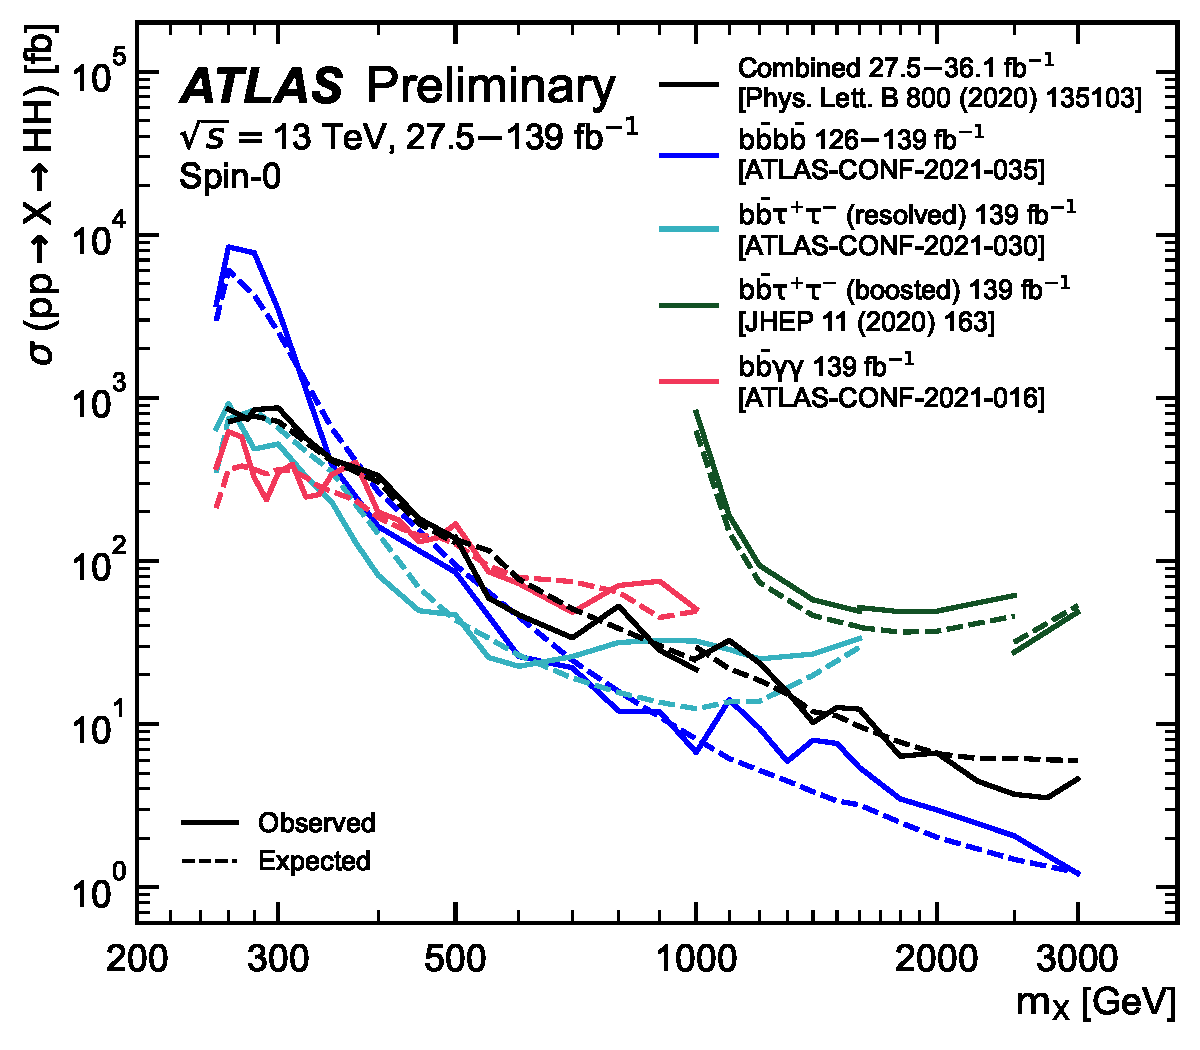
\includegraphics[width=0.8\textwidth]{figures/full-run2-summary-res.pdf}
		 }

\caption{\label{fig:res-comparison} Comparison of full Run 2 ATLAS $HH$ searches for spin-0 resonances. The \bbbb 
channel (blue) is compared with full Run 2 results from $b\bar{b}\tau^{+}\tau^{-}$ (both resolved and boosted) and  
$b\bar{b}\gamma\gamma$, as well as the combined early Run 2 results. The \bbbb channel has leading sensitivity above 
a mass of around \SI{700}{\GeV}, and is competitive with other channels across much of the mass range, demonstrating 
a strong contribution to the ATLAS $HH$ experimental results.~\cite{ATL-PHYS-PUB-2021-031}}
\end{figure}

\begin{figure}[ht]
\centering
\subfloat{
		  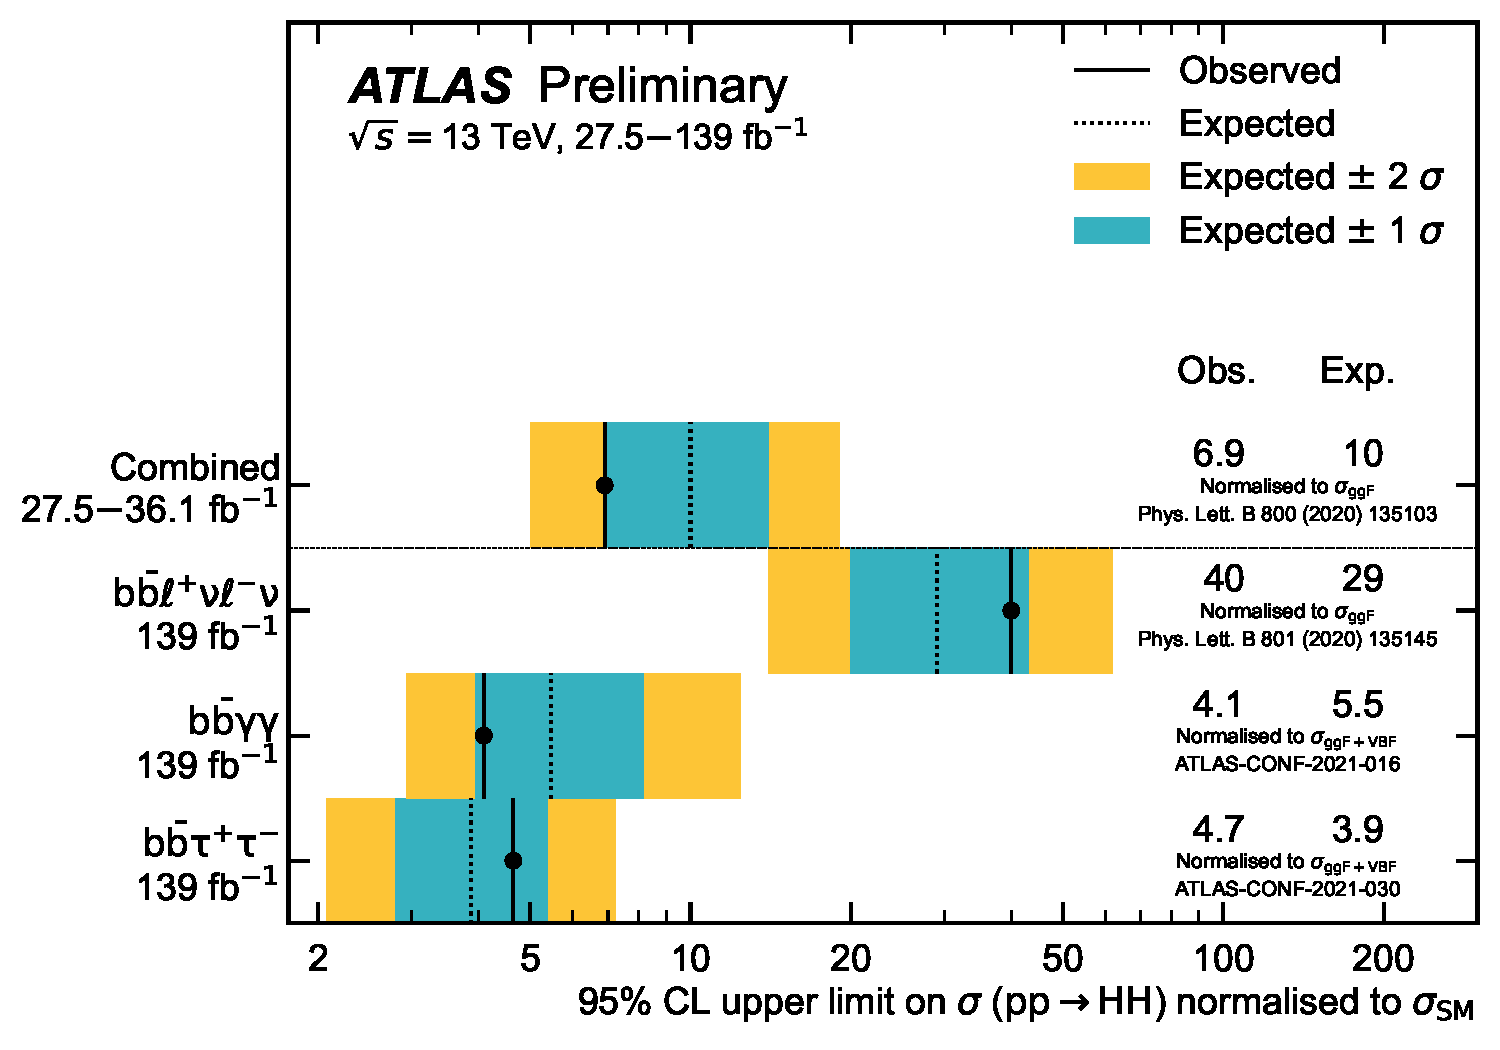
\includegraphics[width=0.8\textwidth]{figures/full-run2-summary-non-res.pdf}
		 }

\caption{\label{fig:nonres-comparison} Comparison of full Run 2 ATLAS $HH$ searches for Standard Model $HH$ production. 
The preliminary results presented in this thesis are not yet included in these results. However, the results presented 
in Table \ref{tbl:SM-HH-limits} are quite competitive with the results from $b\bar{b}\tau^{+}\tau^{-}$ and 
$b\bar{b}\gamma\gamma$, two of the ATLAS channels with leading sensitivity in the search for HH. Note that these 
results include signals produced via both gluon-gluon fusion (ggF) and vector boson fusion (VBF), and are normalized as 
such, while the results of this thesis only include (and are normalized to) ggF production ~\cite{ATL-PHYS-PUB-2021-031}}
\end{figure}